% Intended LaTeX compiler: pdflatex
\documentclass[11pt]{article}
\usepackage[utf8]{inputenc}
\usepackage[T1]{fontenc}
\usepackage{graphicx}
\usepackage{longtable}
\usepackage{wrapfig}
\usepackage{rotating}
\usepackage[normalem]{ulem}
\usepackage{amsmath}
\usepackage{amssymb}
\usepackage{capt-of}
\usepackage{hyperref}
\author{Construção de compiladores I}
\date{}
\title{Análise Léxica}
\hypersetup{
 pdfauthor={Construção de compiladores I},
 pdftitle={Análise Léxica},
 pdfkeywords={},
 pdfsubject={},
 pdfcreator={Emacs 28.2 (Org mode 9.7)}, 
 pdflang={English}}
\begin{document}

\maketitle
\section*{Objetivos}
\label{sec:org55d0f00}

\subsection*{Objetivos}
\label{sec:org4f8bc50}

\begin{itemize}
\item Apresentar a linguagem a ser utilizada para exposição
dos conceitos da disciplina.

\item Definir a etapa de análise léxica e apresentar um analisador
léxico ad-hoc para a linguagem considerada.
\end{itemize}
\section*{Linguagem Imp}
\label{sec:org8da295b}

\subsection*{Linguagem Imp}
\label{sec:org9d5cf5c}

\begin{itemize}
\item Linguagem simples utilizada para exposição dos conceitos da disciplina.

\item Permite a análise de problemas recorrentes no projeto de compiladores.
\end{itemize}
\subsection*{Linguagem Imp}
\label{sec:org32e3cbc}

\begin{itemize}
\item Porém, como especificar uma linguagem de programação?
\end{itemize}
\subsection*{Linguagem Imp}
\label{sec:org8884673}

\begin{itemize}
\item Sintaxe definida usando gramáticas livres de contexto.
\begin{itemize}
\item Alguns elementos são descritos por Expressões regulares.
\end{itemize}
\end{itemize}
\subsection*{Linguagem Imp}
\label{sec:orga94f5d9}

\begin{itemize}
\item Elementos \(\mathrm{léxicos}\) são representados utilizando pela string propriamente dita
\begin{itemize}
\item Ex.: \(\mathrm{if}\), \(\mathrm{while}\) e outras palavras reservadas.
\end{itemize}

\item Outros elementos léxicos: identificadores e números.
\end{itemize}
\subsection*{Linguagem Imp}
\label{sec:orgea12361}

\begin{itemize}
\item Identificadores: \(\mathrm{letter(letter + digit)^*}\)
\begin{itemize}
\item \(\mathrm{letter = a + b + c + ... + A + B + ...}\)
\item \(\mathrm{digit = 0 + 1 + ... + 9}\)
\end{itemize}
\end{itemize}
\subsection*{Linguagem Imp}
\label{sec:org2861e1b}

\begin{itemize}
\item Comentários:
\begin{itemize}
\item Linha: \(\textrm{// este é um comentário.}\)
\item Bloco: \(\textrm{/* este é um comentário. */}\)
\end{itemize}
\end{itemize}
\subsection*{Linguagem Imp}
\label{sec:org396e706}

\begin{itemize}
\item Sintaxe de Imp
\end{itemize}

\begin{array}{lcl}
Program   & \to  & Stmts\\
Stmts     & \to & Statement\:\:Stmts\,\mid\,\lambda\\
\end{array}
\subsection*{Linguagem Imp}
\label{sec:org9c679cf}

\begin{itemize}
\item Sintaxe de Imp
\end{itemize}

\begin{array}{lcl}
Statement & \to  & \mathtt{skip ;}\:\:\mid\:\:Type\:\:\mathrm{id}\:\:Init \mathrm{;} \\
          & \mid & \mathrm{id}\:\:\mathtt{:=}\:\:Expr\mathrm{;}\\
          & \mid & \mathtt{read}\:\:\mathrm{id ;}\:\:\mid\:\:\mathtt{print}\:\:Expr \mathrm{;}\\
          & \mid & \mathtt{if}\:\:Expr\:\:\mathtt{then}\:\:Block\\
          & \mid & \mathtt{if}\:\:Expr\:\:\mathtt{then}\:\:Block\:\:\mathrm{else}\:\:Block\\
          & \mid & \mathtt{while}\:\:Expr\:\:Block
\end{array}
\subsection*{Linguagem Imp}
\label{sec:org80e7954}

\begin{itemize}
\item Sintaxe de Imp (Continuação)
\end{itemize}

\begin{array}{lcl}
Expr & \to  & Expr\:\:Op\:\:Expr\\
     & \mid & \mathrm{-}\:\: Expr\:\mid\:\mathrm{(} Expr \mathrm{)}\\
     & \mid & \mathrm{!}\:\: Expr\\
     & \mid & \mathrm{number}\,\mid\, \mathrm{id}\\
     & \mid & \mathrm{true}\,\mid\,\mathrm{false}\\
\end{array}
\subsection*{Linguagem Imp}
\label{sec:org50d3d08}

\begin{itemize}
\item Sintaxe de Imp (Continuação)
\end{itemize}

\begin{array}{lcl}
Op   & \to  & \mathrm{+}\:\mid\:\mathrm{-}\:\mid\:\mathrm{*}\:\mid\:\mathrm{/}\\
     & \mid & \mathrm{\&\&}\:\mid\:\mathrm{<}\:\mid\:\mathrm{==}\\
Type & \to  & \mathrm{int}\,\mid\,\mathrm{bool}\\
Block & \to & \mathrm{\{} Statement^* \mathrm{\}}\\
Init & \to & \mathrm{:=}\:\:Expr\,\mid\,\lambda\\
\end{array}
\section*{Análise léxica}
\label{sec:org1d7c889}

\subsection*{Análise léxica}
\label{sec:org7f28ebb}

\begin{itemize}
\item Primeira etapa do frontend de um compilador.

\item Responsável por dividir a entrada em uma sequência de \textbf{tokens}.
\begin{itemize}
\item Eliminar espaços em branco e comentários.
\end{itemize}
\end{itemize}
\subsection*{Análise léxica}
\label{sec:orgd70d22d}

\begin{itemize}
\item Token: string que pode ser considerada indivisível pela gramática
de uma linguagem.
\end{itemize}
\subsection*{Análise léxica}
\label{sec:orgfeaa30b}

\begin{itemize}
\item Como implementar um analisador léxico para uma linguagem?

\item Intuitivamente, um analisador léxico é uma função de tipo
\end{itemize}

\begin{verbatim}
String -> [Token]
\end{verbatim}
\subsection*{Análise léxica}
\label{sec:orgb35bb08}

\begin{itemize}
\item Representação de tokens
\end{itemize}

\begin{verbatim}
data Token
  = Id String | Number Int | LPAREN | RPAREN
  | PLUS | TIMES | MINUS | DIV | AND | NOT 
  | ASSIGN | SEMI | LT | EQ ...
\end{verbatim}
\subsection*{Análise léxica}
\label{sec:orgeb04cbf}

\begin{itemize}
\item Definir uma função de tipo:
\end{itemize}

\begin{verbatim}
data Result = Begin | Error String | Success [Token]
 
lexer :: String -> Result
lexer = foldr step Begin . concatMap words . lines
\end{verbatim}
\subsection*{Análise léxica}
\label{sec:orgc4d0bac}

\begin{itemize}
\item Continuação\ldots{}
\end{itemize}

\begin{verbatim}
step :: String -> Result -> Result
step _ (Error s) = Error s
step s Begin = case s of
                "if" -> Success [IF]
                "then" -> Success [THEN]
                ...
\end{verbatim}
\subsection*{Análise léxica}
\label{sec:org2fb8f6e}

\begin{itemize}
\item Apesar de possível, essa abordagem possui problemas.
\begin{itemize}
\item Não é escalável.
\item Não é simples eliminar comentários com essa estratégia.
\end{itemize}
\end{itemize}
\subsection*{Análise léxica}
\label{sec:org637f813}

\begin{itemize}
\item Dificuldade com comentários
\begin{itemize}
\item Funções \texttt{lines} e \texttt{words} dividem strings em linhas e palavras.
\item Problema: comentários em bloco.
\end{itemize}
\end{itemize}
\subsection*{Análise léxica}
\label{sec:org866e5ca}

\begin{itemize}
\item Seria possível realizar a análise léxica de forma:
\begin{itemize}
\item Sistemática
\item Escalável
\item Eficiente
\end{itemize}
\end{itemize}
\subsection*{Análise léxica}
\label{sec:org4b177da}

\begin{itemize}
\item A resposta para as perguntas anteriores é \textbf{SIM}

\item Para resolvermos o dilema da análise léxica usaremos:
\begin{itemize}
\item Autômatos finitos determinísticos (AFDs)
\item Expressões regulares (ERs)
\end{itemize}
\end{itemize}
\subsection*{Análise léxica}
\label{sec:org21aa1ae}

\begin{itemize}
\item Intuitivamente:
\begin{itemize}
\item Processamento da entrada usando AFDs.
\item Especificação de lexemas utilizando ERs.
\end{itemize}
\end{itemize}
\section*{Autômatos finitos}
\label{sec:org2a939ae}

\subsection*{Autômatos finitos}
\label{sec:org637b6c4}

\begin{itemize}
\item Um AFD é uma quíntupla \(M=(E,\Sigma,\delta,i,F)\):
\begin{itemize}
\item \(E\): conjunto de estados.
\item \(\Sigma\): alfabeto de entrada.
\item \(\delta\) : E \texttimes{} \(\Sigma\) \(\to\) E: função de transição.
\item \(i\in E\): estado inicial.
\item \(F\subseteq E\): conjunto de estados finais.
\end{itemize}
\end{itemize}
\subsection*{Autômatos finitos}
\label{sec:org88ccf95}

\begin{itemize}
\item Representando um autômato em Haskell
\end{itemize}

\begin{verbatim}
data DFA a
  = DFA {
      start :: a
    , delta :: a -> Char -> a
    , finals :: a -> Bool
    } 
\end{verbatim}
\subsection*{Autômatos finitos}
\label{sec:org70a16ee}

\begin{itemize}
\item Processando uma string em um DFA
\end{itemize}

\begin{verbatim}
deltaStar :: DFA a -> String -> a
deltaStar m = foldl (delta m) (start m)
\end{verbatim}
\subsection*{Autômatos finitos}
\label{sec:org4e2b316}

\begin{itemize}
\item Relembrando:
\end{itemize}

\begin{verbatim}
foldl :: (b -> a -> b) -> b -> [a] -> b
foldl _ v []       = v
foldl f v (x : xs) = foldl (f v x) xs
\end{verbatim}
\subsection*{Autômatos finitos}
\label{sec:org422fa95}

\begin{itemize}
\item Exemplo: Aceitando números.
\end{itemize}

\begin{center}
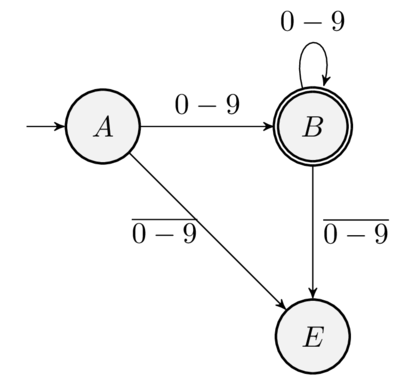
\includegraphics[width=.9\linewidth]{./imgs/image1.png}
\end{center}
\subsection*{Autômatos finitos}
\label{sec:org3eaef01}

\begin{itemize}
\item Exemplo em código Haskell
\end{itemize}

\begin{verbatim}
numberDFA :: DFA (Maybe Bool)
numberDFA
  = DFA {
      start = Just False
    , delta = numberTrans
    , finals = \ e -> e == Just True
    }
    where
      numberTrans (Just False) c
        | isDigit c = Just True
        | otherwise = Nothing
      numberTrans (Just True) c
        | isDigit c = Just True
        | otherwise = Nothing
      numberTrans _ _ = Nothing
\end{verbatim}
\subsection*{Autômatos finitos}
\label{sec:orge2a1efb}

\begin{itemize}
\item Exemplo: aceitando palavras chave
\end{itemize}

\begin{center}
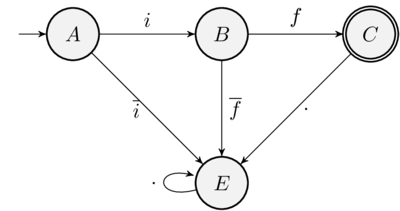
\includegraphics[width=.9\linewidth]{./imgs/image2.png}
\end{center}
\subsection*{Autômatos finitos}
\label{sec:orgefb5cac}

\begin{itemize}
\item Exemplo em código Haskell
\end{itemize}

\begin{verbatim}
ifDFA :: DFA (Maybe Int)
ifDFA
  = DFA {
      start = Just 0
    , delta = ifTrans
    , finals = \ e -> e == Just 2
    }
 where
   ifTrans (Just 0) 'i' = Just 1
   ifTrans (Just 1) 'f' = Just 2
   ifTrans _ _ = Nothing
\end{verbatim}
\subsection*{Autômatos finitos}
\label{sec:org58246ca}

\begin{itemize}
\item Problema: lexemas da linguagem não são disjuntos.
\begin{itemize}
\item Considere os tokens \(\mathrm{if}\) e \(\mathrm{iftrue}\)
\item Como um AFD deve lidar com essa situação?
\end{itemize}
\end{itemize}
\subsection*{Autômatos finitos}
\label{sec:org0678136}

\begin{itemize}
\item O analisador léxico deve considerar como token o \textbf{maior prefixo consumido}.

\item Logo, entre \(\mathrm{if}\) e \(\mathrm{iftrue}\), deverá ser escolhido o segundo.
\begin{itemize}
\item Como processar o maior prefixo possível?
\end{itemize}
\end{itemize}
\subsection*{Autômatos finitos}
\label{sec:org7cd0f34}

\begin{itemize}
\item Obtendo o maior casamento em um AFD

\item Função: \textbf{go}
\begin{itemize}
\item 1o argumento: Estado atual.
\item 2o argumento: Tripla formada por:
\begin{itemize}
\item Último estado é final?
\item Prefixo processado e sufixo restante.
\end{itemize}
\end{itemize}
\end{itemize}

\begin{verbatim}
longest :: DFA a -> String -> Maybe (String, String)
longest m s
  = go (start m) (finals m (start m), Just "", Just  s)
\end{verbatim}
\subsection*{Autômatos finitos}
\label{sec:orgaeefdb5}

\begin{itemize}
\item Definição de \texttt{go}.

\item Caso 1: String completamente processada.
\end{itemize}

\begin{verbatim}
go _ (True, Just pre, Just "") = Just (pre, "")
go _ (False, _, Just "") = Nothing
\end{verbatim}
\subsection*{Autômatos finitos}
\label{sec:orgbdf5076}

\begin{itemize}
\item Definição de \texttt{go}

\item Caso 2: Casamento já encontrado.
\end{itemize}

\begin{verbatim}
go e (True, Just pre, Just (c : cs))
  | finals m (delta m e c) = go (delta m e c) (True, Just (c : pre), Just cs)
  | otherwise   = Just (pre, (c : cs))
\end{verbatim}
\subsection*{Autômatos finitos}
\label{sec:org01565a5}

\begin{itemize}
\item Definição de \texttt{go}

\item Caso 3: Casamento ainda não encontrado
\end{itemize}

\begin{verbatim}
go e (False, Just pre, Just (c : cs))
  | finals m (delta m e c) = go (delta m e c)(True, Just (c : pre), Just cs)
  | otherwise = go (delta m e c) (False, Just (c : pre), Just cs)
\end{verbatim}
\subsection*{Autômatos finitos}
\label{sec:orge931927}

\begin{itemize}
\item Como processar todos os tokens de uma entrada?
\end{itemize}

\begin{verbatim}
lexer :: DFA a -> (String -> Maybe [b]) -> String -> Maybe [b]
lexer _ _ "" = return []
lexer m action s
  = do
      (pref, suf) <- longest m s
      token <- action (reverse pref)
      tokens <- lexer m action suf
      return (token ++ tokens)
\end{verbatim}
\subsection*{Autômatos finitos}
\label{sec:org76c6bb6}

\begin{itemize}
\item Pergunta: como combinar os AFDs para\ldots{}
\begin{itemize}
\item Palavras chaves
\item Identificadores
\end{itemize}
\end{itemize}
\subsection*{Autômatos finitos}
\label{sec:org96b7a68}

\begin{itemize}
\item Vamos utilizar a construção da união de AFDs.
\begin{itemize}
\item União definida em termos de produto
\end{itemize}
\end{itemize}
\subsection*{Autômatos finitos}
\label{sec:org18df0ab}

\begin{itemize}
\item Construção de produto
\end{itemize}

\begin{verbatim}
dfaProduct :: (Eq a, Eq b) => DFA a ->
                              DFA b ->
                              ((a,b) -> Bool) -> DFA (a, b)
dfaProduct m1 m2 fin
  = DFA {
      start = (start m1, start m2)
    , delta = delta'
    , finals = fin
    }
    where
      delta' (e1,e2) c = (delta m1 e1 c, delta m2 e2 c)  
\end{verbatim}
\subsection*{Autômatos finitos}
\label{sec:orgfee9b2c}

\begin{itemize}
\item Definindo a união
\end{itemize}

\begin{verbatim}
unionDFA :: (Eq a, Eq b) => DFA a -> DFA b -> DFA (a,b)
unionDFA m1 m2 = dfaProduct m1 m2 g
  where
    g (e1, e2) = finals m1 e1 || finals m2 e2
\end{verbatim}
\subsection*{Autômatos finitos}
\label{sec:org1c4a74a}

\begin{itemize}
\item Resolvendo o problema entre ``if'' e ``ifblabla''.
\end{itemize}

\begin{verbatim}
ifOrIdentDFA :: DFA (Maybe Int, Maybe Int)
ifOrIdentDFA = unionDFA ifDFA identDFA
\end{verbatim}
\section*{Concluindo}
\label{sec:org5750917}

\subsection*{Concluindo}
\label{sec:org8434d0d}

\begin{itemize}
\item Apresentamos a linguagem IMP que será usada neste curso.

\item Discutimos como implementar análise léxica.
\end{itemize}
\subsection*{Concluindo}
\label{sec:orge2ba5c2}

\begin{itemize}
\item Mostramos que AFDs são um formalismo apropriado para denotar
analisadores léxicos.

\item Próxima aula: Especificando lexemas utilizando expressões regulares.
\end{itemize}
\section*{Exercícios}
\label{sec:org8d4f732}

\subsection*{Exercícios}
\label{sec:orgb4a3b52}

\begin{itemize}
\item Utilize as implementações de AFDs para criar um analisador léxico para a linguagem IMP.
Seu programa deve processar um programa de entrada e imprimir a lista de tokens reconhecidos.
\end{itemize}
\end{document}